% Manuel Lippert - Paul Schwanitz
% Physikalisches Praktikum

% Teilaufgabe 2
% TODO: #23 FzV 2.2 @ManeLippert

\section{Das invertierte Pendel}
\label{sec:invertPendel}
Das invertierte Pendel besitzt eine unten fest eingespannte Blattfeder mit Federkonstante $k$, welche über zwei horizontal in der Höhe $h$ und der Auslenkung $x_h$ angreifende Spiralfedern mit Federkonstante $k_s$ un der Auslenkung $\hat{x}$ angetrieben wird. Am oberen Ende der Blattfeder lässt sich ein Zusatzgewicht $M$ anbringen und der Winkel $\theta$ beschreibt den Winkel zwischen der Tangenten an der Pendelspitze und dem Lot. Weiterhin bezeichnet die Pendellänge $L$ die Länge zwischen dem Anfang und Ende der Blattfeder, welche vom Winkel $\theta$ abhängt (siehe \ref{image:invertiertesPendel}).
\begin{center}
    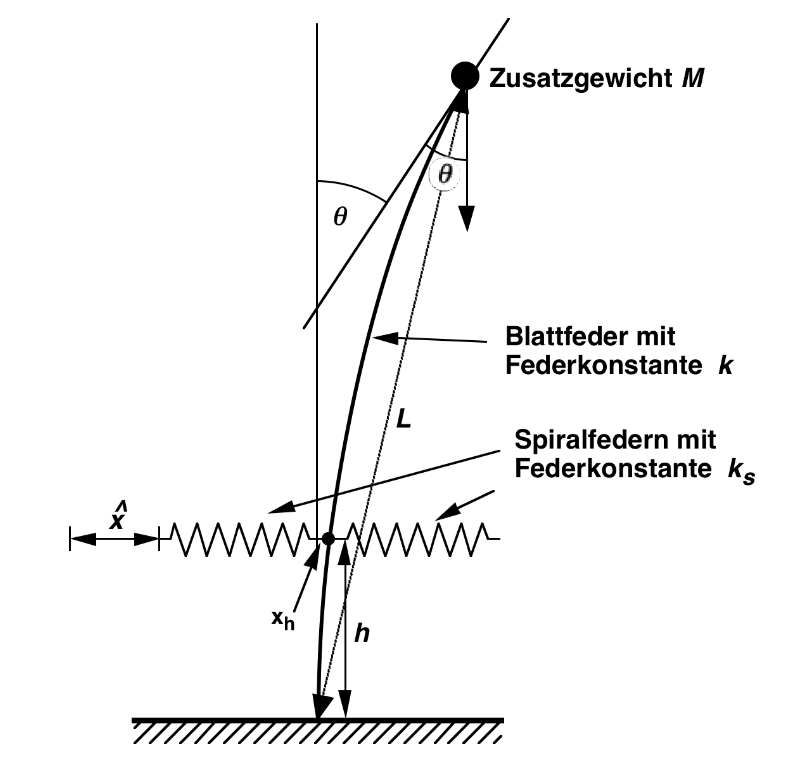
\includegraphics[scale=0.3]{invertiertesPendel.png}
    \captionof{figure}{Skizze invertiertes Pendel}
    \label{image:invertiertesPendel}
\end{center}
\subsection{Herleitung der Bewegungsgleichung}
\label{sub:bewegungsgleichung}
Die Bewegungsgleichung lässt sich über die wirkenden Drehmomente der Bauteile bestimmen:
\begin{gather*}
        \text{Pendel}~+~\text{Dämpfung}~+~\text{Blattfeder}~-~\text{Spiralfedern}~-~\text{Gewicht} = 0
\end{gather*}
\begin{gather}
    \Rightarrow [M(L(\theta))^2\ddot{\theta}]+[2c\dot{\theta}]+[k\theta]-[hk_s(x_h+\hat{x}\cos(\omega_at))]-[MgL(\theta)\sin(\theta)]=0
\end{gather}
Dabei bezeichnet $c$ die Dämpfungskonstante und $g$ die Erdbeschleunigung.\\
Im Folgenden wird die Pendellänge $L$ als konstant angenommen, obwohl dieser nicht konstant ist und von der Art der verwendeten Masse $M$ abhängt. Weiterhin wird die Auslenkung $x_h$ als vernachlässigbar klein angesehen und der Angriffswinkel der Spiralfedern wird als $\frac{\pi}{2}$ genähert, was bei genügend kleiner Höhe $h$ gegeben ist.
Daraus folgt die genäherte Form der Bewegungsgleichung:
\begin{gather}
    ML^2\ddot{\theta}+2c\dot{\theta}+k\theta-MgL(\theta)\sin(\theta)=hk_s\hat{x}\cos(\omega_at)=T_0\cos(\omega_at)
\end{gather}
Wobei $T_0$ als die Amplitude des periodisch angreifenden Drehmoments interpretiert werden muss.

\subsection{Schwingungsdauer in Abhängigkeit der Masse}
\label{sub:schwingungsdauer}

\subsection{Symmetriebrechung}
\label{sub:symbrechung}

\subsection{Differenzier-Schaltung}
\label{sub:diffSchaltung}
% Sie Versuch EL2